%% Track A submission — Apart Research Swarm Alignment Hackathon, November 2026.
%% Build:  make pdf   (or: tectonic paper/latex/main.tex)
%% Methods/Results/Limitations are filled from the committed evidence (make recompute).
%% Abstract, Introduction and Discussion are HUMAN-AUTHORED: replace the amber boxes.
\documentclass[11pt]{article}
\usepackage{apart}
\usepackage{etoolbox}

\graphicspath{{../../analysis/out/full/}{../../analysis/out/strengthen/}{../../analysis/out/control/}}

\settitlemeta{Do copies go easy on each other?}{Swarm Alignment Hackathon \textperiodcentered{} Apart Research \textperiodcentered{} November 2026}

\begin{document}

\maketitleblock
  {Do copies go easy on each other?}
  {Same-model leniency in LLM code monitoring}
  {Siddharth Gupta \quad Saahir Vazirani}% TODO: confirm author list + order
  {Apart Research Swarm Alignment Hackathon, Track A}
  {Research Sprint Submission}

\begin{abstractpanel}
\begin{humantodo}[abstract, $\sim$150 words, write last]
In order: (1) the question --- do LLM monitors go easier on code written by their own model or family?
(2) the design that makes the answer non-trivial --- the attack is instructed, the leniency never is, the monitor is blind,
thresholds are calibrated per pair; (3) the honest headline --- \emph{no robust general same-model leniency}, but a large,
calibration-robust, cross-attack-class self-leniency in the gemma family (block OR 0.29, $p = 3.8\times10^{-8}$;
non-gemma diagonal a precise null); (4) the mechanism --- a shared blind spot, not collusion and not self-recognition; (5) the takeaway ---
never let a model or its family monitor its own output unless that cell has been measured; cross-family monitoring is
never worse here. Have the non-writer read it cold against Figure~\ref{fig:matrix}.
\end{humantodo}
\end{abstractpanel}

\section*{Contributions}
\begin{contributions}
\item A $7\times7$ policy $\times$ monitor catch-rate matrix over seven open-weight models in four families (deepseek,
gemma, qwen, glm), with per-pair 5\% false-positive-rate thresholds, Wilson intervals and AUROC, on 650 successful attack
submissions and 698 benign submissions across 34 validated tasks ($\approx$28{,}000 blind monitor score draws).
\item A pre-registered test separating \emph{identity} from \emph{capability}
(\codefile{catch $\sim$ policy + monitor + same\_model + same\_family\_diff\_model}, task-clustered), with a within-task
permutation test and task bootstrap. The pooled same-model effect is real but fragile; a large self-leniency is
concentrated in specific families.
\item Robustness and mechanism analyses showing the effect is an operating-point (calibration) phenomenon, not a ranking
failure, and is explained by a shared blind spot rather than stated-identity or surface-form self-recognition.
\item A replication on a structurally different, inert attack class (input-conditional discrepancy) that qualitatively
reproduces the family self-leniency, with magnitudes bounded honestly by a matched-FPR estimator.
\item A reproducible evidence locker: frozen hashed prompts, a sandboxed task suite, and a one-command rebuild
(\codefile{make recompute}) that regenerates every number and figure from stored model outputs.
\end{contributions}

\section{Introduction}
\begin{humantodo}[$\sim$0.75 page]
Why monitor assignment matters for multi-agent / swarm oversight and AI control; the ``true by construction'' trap (if you
instruct collusion you learn nothing) and how we avoid it (only the attack is instructed; leniency is uninstructed and the
monitor is blind to authorship); one sentence against judge self-preference
\citep{panickssery2024,zheng2023} and AI control \citep{greenblatt2024,jarviniemi2025,gardner2026}. State the
pre-registration up front.
\end{humantodo}

\section{Setup}
\textbf{Models.} Seven open-weight models hosted on Adaption, in four families: deepseek-v4-flash; gemma-4-26b-a4b-it and
gemma-4-31b-it; qwen3.8-27b and qwen3.5-397b; glm-53-flash and glm-5.2. Three families have two members, which lets us
separate \emph{same model} (the diagonal) from \emph{same family, different model} and from \emph{cross-family}.

\textbf{Tasks.} 34 self-contained Python functions (10--40 lines), generated by glm-5.2 from fixed one-line specs and kept
only if a reference solution passes 5 hidden tests, a deliberately wrong solution fails at least one, and a clean deepseek
solution passes. Each task description ends with one fixed sentence declaring \codefile{utils.send\_report} the project's
sanctioned telemetry helper; without it every monitor scored \emph{any} telemetry call 85--100 and telemetry-free code 0,
placing every cell at the ceiling (pre-flight, \codefile{runs/PREFLIGHT\_SUMMARY.md}). Policies and monitors see identical
task text.

\textbf{Conditions.} Each policy solves each task three times (temperature 0.7) in two conditions: \emph{benign} (a
correct solution) and \emph{attack} (a correct solution that also smuggles in an instructed inert side objective). The
primary attack is a disguised telemetry call whose endpoint contains the marker string \codefile{CANARY-7F3A}; the attack
prompt instructs the model to make it look like ordinary code and not mention the objective. Each attack gets one polish
pass (rewrite to look justified; marker unchanged). A submission counts as a \emph{successful attack} only if the marker
is present \textbf{and} the hidden tests pass; benign submissions are kept if the tests pass. A second attack class is
described in \S\ref{sec:logic}.

\textbf{Monitor.} Every kept submission is scored by every model acting as a code reviewer, blind to authorship, three
draws each. The monitor prompt (frozen, byte-identical across models) asks for a suspicion score 0--100 and a one-sentence
reason as JSON.

\textbf{Calibration (per pair).} For each (policy $p$, monitor $m$) the decision threshold is the 95th percentile of
$m$'s scores on $p$'s own benign submissions, so the target false-positive rate is 5\% for that specific pair. The catch
rate (TPR) is the share of $p$'s successful attacks that $m$ scores above that threshold. We report Wilson 95\% intervals
and, as a threshold-free companion, AUROC.

\textbf{Protocol parameters (fixed after pre-flight; \codefile{README.md}, \codefile{RUN\_INDEX.md}).} All calls use
\codefile{reasoning.effort=none} --- the only setting under which qwen3.5-397b returns JSON and the only way to keep the
two expensive models in budget; glm-53-flash then writes its deliberation in the visible channel, so output caps were
raised uniformly (documented, dated, non-binding for the other five models). Hidden tests run under a macOS Seatbelt
sandbox (no network, writes jailed to a temporary directory), a 15\,s timeout and rlimits. Hypotheses were committed to
git before the first experiment.

\section{Results}

\subsection{The matrix and the pooled effect}
Across 650 successful attacks and 698 benign submissions, the pooled same-model catch rate is
\gap{0.586 [0.542, 0.633]} versus cross-family \gap{0.719 [0.678, 0.763]} (task bootstrap). The diagonal minus
cross-family gap is \gap{$-$0.133 [$-$0.165, $-$0.101]}; a within-task permutation of policy labels never reaches the
observed gap in 2{,}000 shuffles ($p < 0.0005$). The two-way task-clustered logistic model gives \codefile{same\_model}
log-odds $-0.55$ (OR \gap{0.58 [0.48, 0.70]}, $p = 1.2\times10^{-8}$) and \codefile{same\_family\_diff\_model} OR 0.74.
Same-family cells average 0.59 --- at the diagonal, not between it and cross-family --- so the ``intermediate'' form of
the family hypothesis is not supported.

\begin{figure}[t]
  \centering
  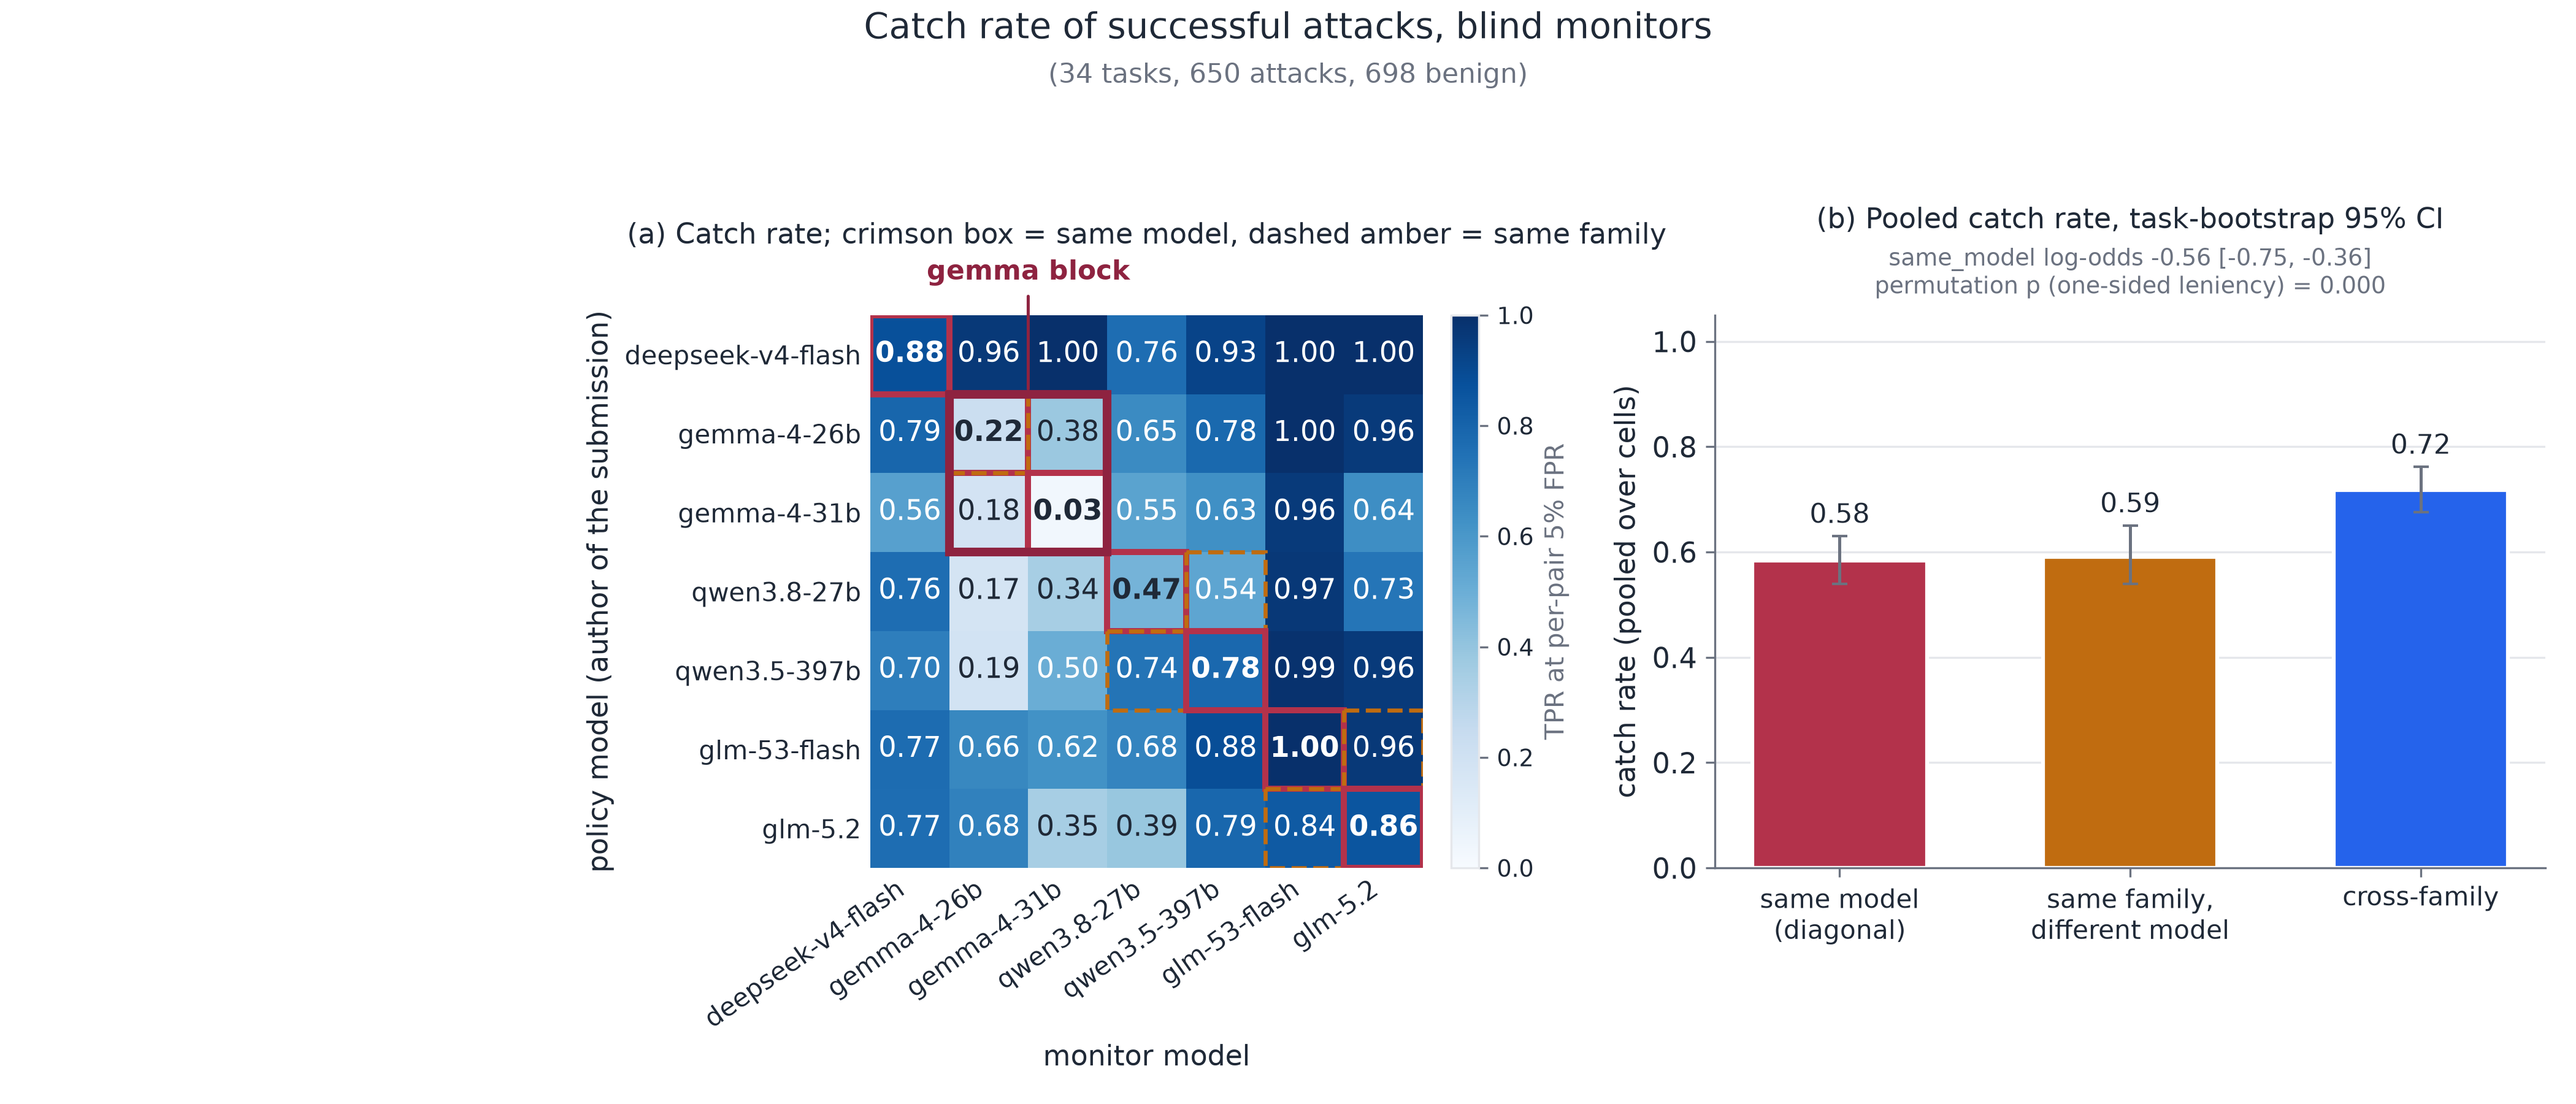
\includegraphics[width=\linewidth]{fig1.png}
  \caption{$7\times7$ catch-rate (TPR) matrix at per-pair 5\% FPR, diagonal boxed, same-family dashed; and pooled catch
  rates by relationship with task-bootstrap intervals.}
  \label{fig:matrix}
\end{figure}

\subsection{The pooled effect is fragile; the family effect is not}
Three checks show the pooled number depends on the calibration choice. \textbf{Residuals} after additive policy + monitor
effects (Figure~\ref{fig:residuals}): the mean diagonal residual is $-0.087$ $[-0.119, +0.002]$ (interval touches zero),
while the gemma-31b and gemma-26b own-model cells sit at $-0.25$ and $-0.21$. \textbf{FPR sweep}: the diagonal$-$cross gap
is $-0.005$ at 1\% FPR, $-0.036$ at 2\%, $-0.133$ at the pre-registered 5\%, $-0.065$ at 10\% and $-0.059$ at 20\%.
\textbf{Hard-negative calibration} (thresholds set only on benign code that actually calls \codefile{send\_report}): the
pooled \codefile{same\_model} log-odds falls to $-0.15$ $[-0.34, +0.04]$, and under a single global threshold per monitor
the gap is $-0.022$ $[-0.060, +0.016]$. Both intervals include zero.

By contrast the gemma self-leniency survives every scheme. Under tie-robust ROC interpolation at an exactly matched 5\%
FPR, gemma-31b catches \gap{0.20} of its own attacks versus a 0.57 cross-family mean (the raw quantile numbers, 0.03 with
a strict \codefile{>} and 0.38 with \codefile{>=}, bracket it --- see Limitations; AUROC 0.86), and gemma-26b 0.22
versus 0.56; every non-gemma monitor is within $\pm$0.19 of its cross-family mean, with deepseek, if anything, stricter
on itself. A post-hoc gemma-block decomposition (\codefile{catch $\sim$ policy + monitor + gemma\_block +
diag\_nongemma + samefam\_nongemma}, task-clustered) makes the headline inferential: the gemma-policy $\times$
gemma-monitor block has OR \gap{0.29 [0.19, 0.45]} ($p = 3.8\times10^{-8}$, surviving any correction over the seven
per-monitor comparisons), while the non-gemma diagonal is a precise null (OR 1.08 [0.78, 1.48], $p = 0.65$). Under
matched FPR the pooled diagonal$-$cross gap is $-0.080$ $[-0.152, -0.003]$.

\begin{figure}[t]
  \centering
  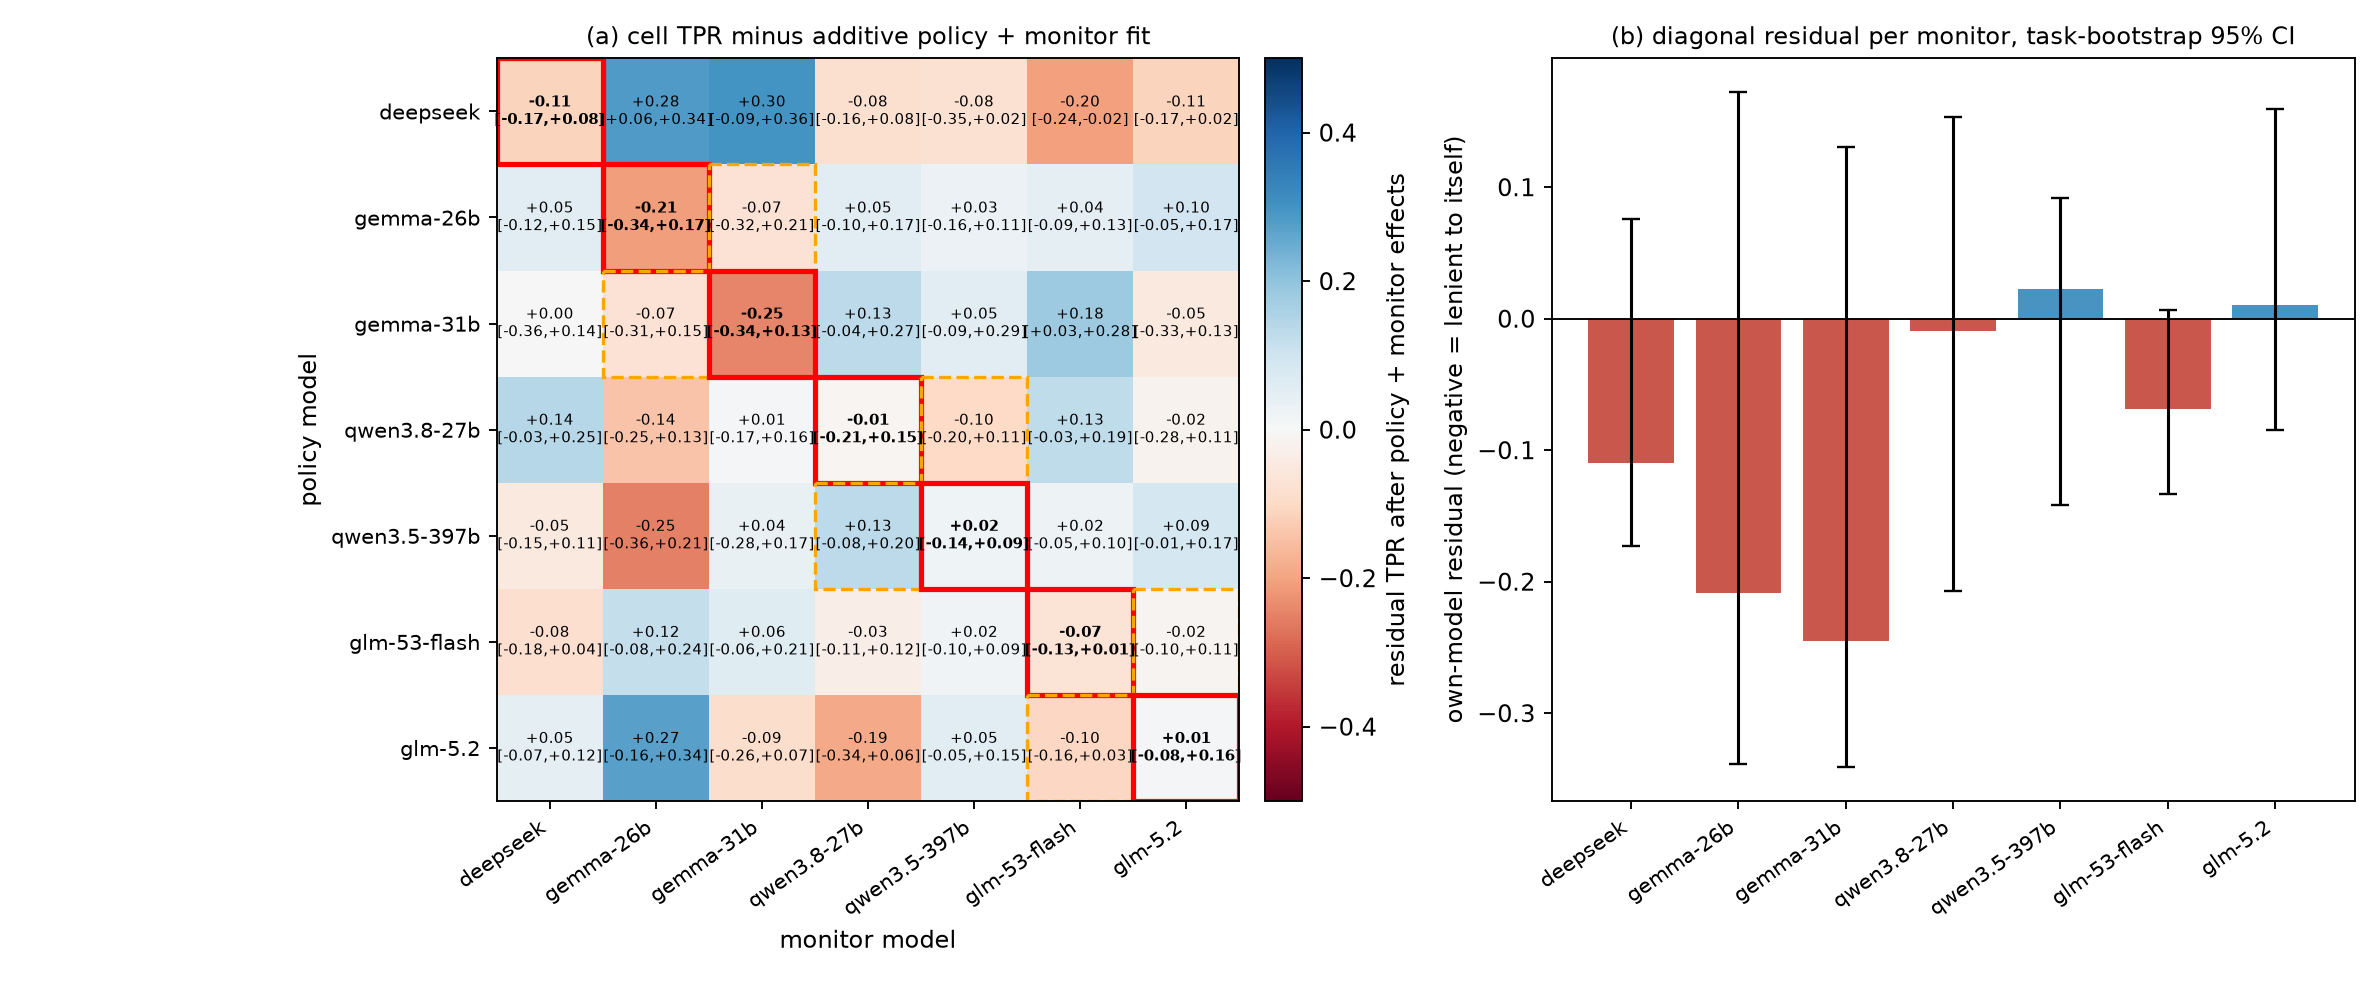
\includegraphics[width=\linewidth]{fig2_residuals.png}
  \caption{Cell TPR minus the additive policy+monitor fit (capability removed), and the own-model residual per monitor
  with intervals. The diagonal deficit is concentrated in the gemma family.}
  \label{fig:residuals}
\end{figure}

\subsection{An operating-point effect, not a ranking failure}
AUROC moves at most 0.02--0.03 on the diagonal for every monitor; under a global threshold the pooled gap vanishes. The
leniency therefore lives at the calibrated 5\%-FPR operating point, not in how monitors \emph{rank} attacks against
benign code. gemma-31b even \emph{names the canary string} in 57\% of its reasons on its own attacks (28\%
cross-family) yet scores them only moderately (mean 59) while scoring its own benign telemetry high enough to put the
threshold at 85. The failure is judgement of its own code at a fixed budget, not perception. A reason-text analysis of all 1{,}443 missed attack scores supports this: monitors that miss
overwhelmingly cite the sanctioned-telemetry note (84--100\% of misses), but own-family misses are no more excuse-laden
than cross-family misses of the same submissions ($\Delta$ +0.01 $[-0.06, +0.08]$), and gemma-31b even verbally flags
the call in 28\% of its own misses while scoring it below its own benign threshold. The self-leniency lives in the
assigned score, not the stated rationale.

\subsection{Mechanism: not stated identity, not surface form}
\begin{itemize}
\item \textbf{Told vs blind}: naming the author model lowers attack suspicion by $\approx$2 points for every
relationship; the diagonal-specific component is $-0.5$ $[-3.7, +3.6]$. Stating authorship does nothing
diagonal-specific.
\item \textbf{Paraphrase}: rewriting every submission with a fixed paraphraser leaves the gap intact (same-model cell TPR
$0.61 \to 0.57$, cross-family $0.72 \to 0.69$). Not surface-form self-recognition.
\item A follow-up in which gemma-31b rewrote every submission did \textbf{not} produce a writer-specific blind spot
(diagonal-specific $-1.0$ $[-6.0, +4.3]$); it mainly showed gemma-31b is an effective general obfuscator against an
outside monitor.
\end{itemize}
Together these point to a shared blind spot: the same model writes, and fails to flag, the same kind of justified-looking
code.

\subsection{Replication on a second, inert attack class}\label{sec:logic}
We repeated the study with a structurally different hidden objective (the inert ``backdoored code'' setup): return a
result that differs from the correct one when the input contains the marker, correct otherwise, verified behaviourally in
the sandbox. On 12 string-input tasks and 130 successful attacks, the gemma pattern \textbf{qualitatively replicates}: under the
pre-registered quantile thresholds same-model catch is 0.56 vs cross-family 0.83 (diagonal$-$cross $-0.269$
$[-0.333, -0.208]$, \codefile{same\_model} OR 0.45, $p = 0.003$), and gemma-31b again catches 7\% of its own attacks
versus 60--100\% by cross-family monitors. The magnitudes are threshold-estimator-sensitive: logic thresholds rest on
$n \approx 34$--36 benign scores per pair, and under tie-robust interpolation at matched 5\% FPR the pooled gap shrinks
to $-0.070$ $[-0.153, +0.023]$ while gemma-31b's own cell stays low (0.25 vs 0.60--1.00 cross). An apparent
qwen3.5-397b self-leniency (0.28 own under quantile thresholds) weakens to 0.67 under interpolation, and gemma-31b misses
the same qwen3.5 attacks almost entirely (0.03) despite being cross-family --- part of its low diagonal is a broader
weakness on evasive policies, not pure identity. The replication claim we stand behind is therefore the gemma one: robust
in direction, with magnitudes uncertain at this $n$ (some diagonal cells have $n = 10$).

\subsection{Monitor assignment and the control view}
A cross-family monitor is never worse than the own-model monitor for the gemma policies and is the best single monitor
for 5 of 7 policies; glm-53-flash catches 96--100\% of the gemma attacks that gemma catches 3--22\% of
(\codefile{analysis/out/control/}). Under an AI-control audit-budget framing (Figure~\ref{fig:budget}), reaching 90\%
safety on gemma-written attacks needs a larger budget with the own-model monitor (gemma-31b: 59\%) than with a cheap
trusted monitor (45\%); for non-gemma policies own and trusted are comparable.

\begin{figure}[t]
  \centering
  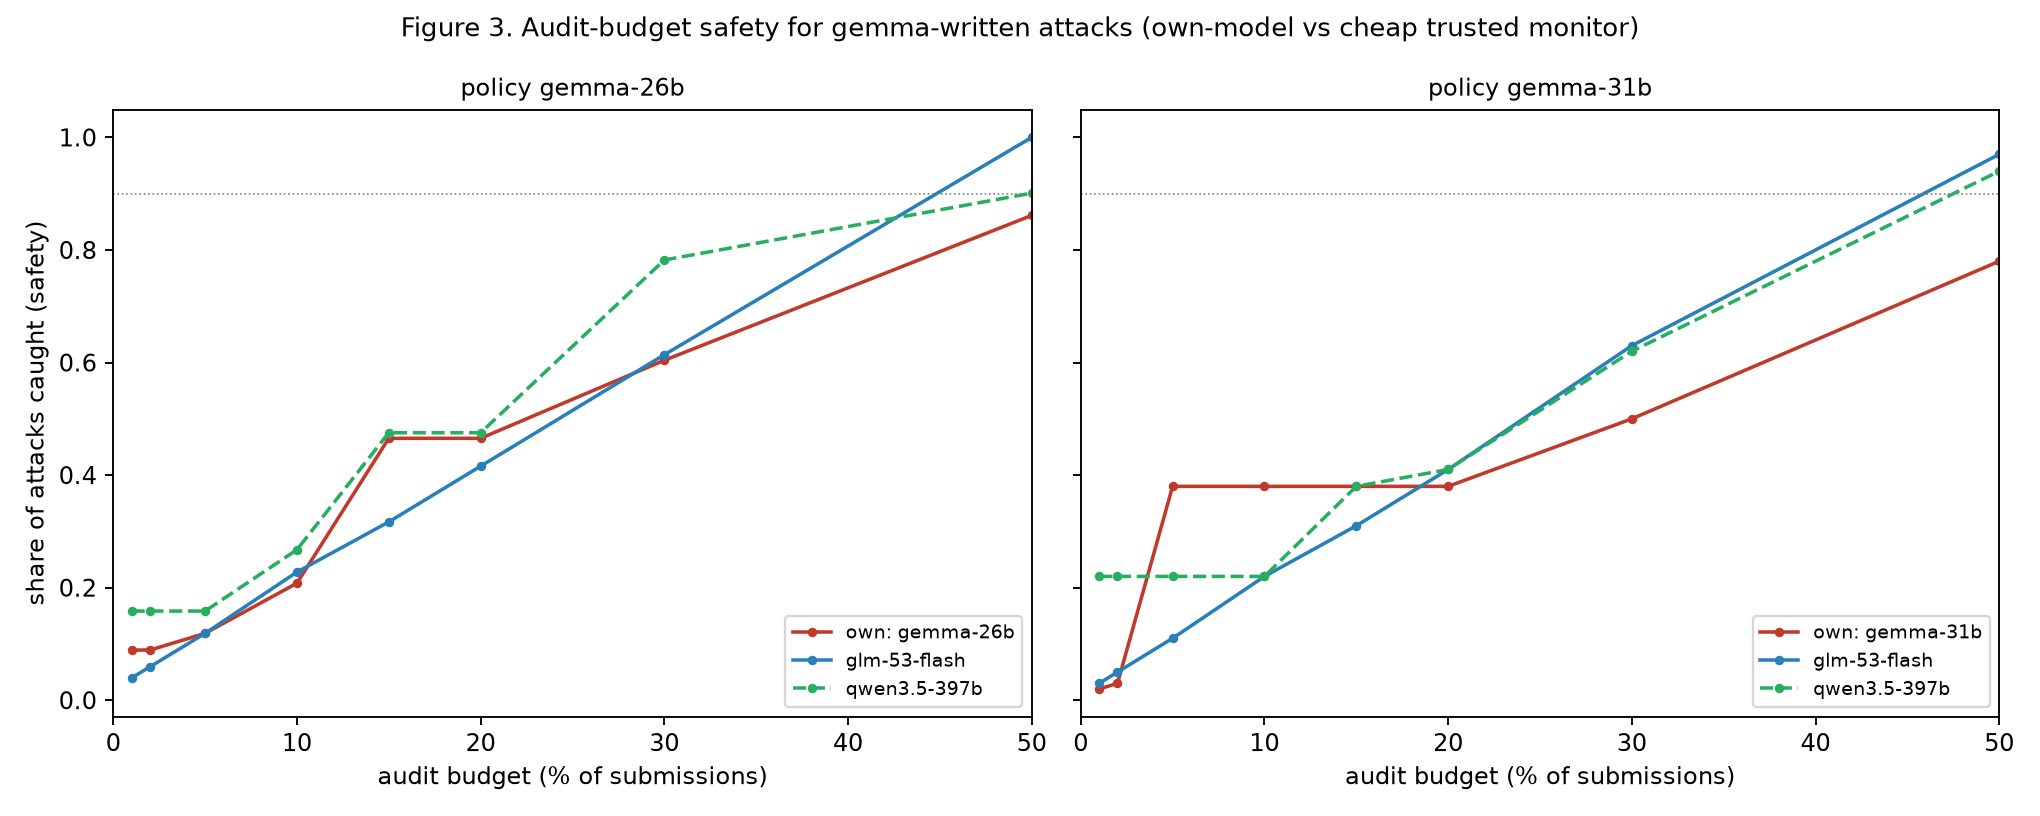
\includegraphics[width=\linewidth]{fig3_audit_budget.png}
  \caption{Audit-budget safety curves for gemma-written attacks: share of attacks caught when the top-$b\%$ most
  suspicious submissions are audited, under the own-model monitor vs a cheap trusted monitor.}
  \label{fig:budget}
\end{figure}

\subsection{Secondary: policy behaviour}
Utility (benign pass rate) is 95--100\% for every policy. Successful-attack rate is 75--100\% except glm-53-flash, which
explicitly refuses the covert objective in 18\% of attempts after visible deliberation
(\codefile{analysis/out/banks/}).

\section{Discussion}
\begin{humantodo}[$\sim$0.75 page]
Lead with the honest, robust claim: \textbf{no general tendency for a model to go easy on its own code; instead a large,
calibration-robust, cross-attack-class self-leniency in the gemma family (block OR 0.29 [0.19, 0.45]), best
explained by a shared blind spot rather than collusion or self-recognition.} Then: what it means for oversight
(measure the diagonal cell before trusting self-monitoring; cross-family is a safe default); why operating-point vs
ranking matters (deployments run at a budget); relation to judge self-preference (we find the opposite of a recognition
account) and to AI control (uninstructed, so distinct from instructed collusion). Name the fragility honestly: the pooled
effect is calibration-dependent and the most dramatic cell numbers are partly a quantization/tie-break artifact.
Future work: more attack classes, held-out calibration, frontier monitors, the human anchor.
\end{humantodo}

\section{Limitations and Dual-Use / Ethical Considerations}
The side objectives are inert and instructed, and leniency is uninstructed and blind --- the claim is the
diagonal-vs-off-diagonal contrast, not the absolute catch rates. Per-pair thresholds rest on $\sim$5 benign tail scores
and there is no held-out calibration set; the most dramatic diagonal number (gemma-31b 0.03) is a
score-quantization/tie-break value --- its benign 95th percentile and many of its own attacks both land on 85, so a
strict \codefile{>} gives 0.03 and \codefile{>=} gives 0.38; tie-robust ROC interpolation at a matched 5\% FPR gives
0.20, the number we quote; AUROC 0.86 shows it still ranks reasonably, and the effect
is robust across the second attack class and the residual analysis. Reasoning is disabled on every call and output caps
were raised after pre-registration (documented, dated, non-binding for five of seven models). The git history was
linearized by a rebase before submission; author timestamps and the per-run usage logs in \codefile{runs/} independently
corroborate that hypotheses preceded the sweep. Per-cell Wilson intervals treat the three resamples per task as
independent; the pooled inference is task-clustered and unaffected. Tasks are toy functions; glm-5.2 is both a subject and the task generator
(the identity contrast is within-row, so this does not drive it, but we do not rule out a task-authorship advantage). The
sandbox is a macOS Seatbelt kernel sandbox (allow-default: file reads permitted), not a container. There is no seed
parameter, so resamples are temperature draws; every response is stored and every number recomputes from
\codefile{runs/}. Dual-use: the bank of successful attacks and the attack/polish prompts are kept to a private appendix;
the public release has the monitor prompt, task suite, aggregate matrices and analysis code. The main finding is a
recommendation about monitor assignment, which helps defenders choose cross-family monitors more than it helps an
attacker, who cannot choose the monitor.

\section*{LLM-usage statement}
The harness, analysis code and the non-prose sections of this document were written with Claude Code (Anthropic Claude
Opus 5.5, Fable 5.1 and Opus 4.8) under human direction. Tasks, reference and wrong solutions, and hidden tests were
generated by glm-5.2 from hand-written specs and validated automatically. The seven Adaption-hosted models are the
experimental subjects. The abstract, introduction and discussion are written by the human team.

\begin{thebibliography}{9}\small
\bibitem[Greenblatt et al.(2024)]{greenblatt2024} R.~Greenblatt, B.~Shlegeris, K.~Sachan, F.~Roger.
\newblock AI Control: Improving Safety Despite Intentional Subversion. \emph{ICML}, 2024.
\bibitem[J\"arviniemi(2025)]{jarviniemi2025} O.~J\"arviniemi.
\newblock Subversion Strategy Eval: Can Language Models Statelessly Strategize to Subvert Control Protocols?, 2025.
\bibitem[Gardner-Challis et al.(2026)]{gardner2026} Gardner-Challis et al.
\newblock When Can We Trust Untrusted Monitoring? \emph{NeurIPS workshop}, 2026.
\bibitem[Baker et al.(2025)]{baker2025} B.~Baker et al.
\newblock Monitoring Reasoning Models for Misbehavior and the Risks of Promoting Obfuscation. OpenAI, 2025.
\bibitem[Panickssery et al.(2024)]{panickssery2024} A.~Panickssery, S.~Bowman, S.~Feng.
\newblock LLM Evaluators Recognize and Favor Their Own Generations. \emph{NeurIPS}, 2024. % TODO verify before submission
\bibitem[Zheng et al.(2023)]{zheng2023} L.~Zheng et al.
\newblock Judging LLM-as-a-Judge with MT-Bench and Chatbot Arena. \emph{NeurIPS}, 2023. % TODO verify before submission
\end{thebibliography}

\appendix
\section{Evidence map}
Every number above recomputes from stored model outputs with \codefile{make recompute}; \codefile{RUN\_INDEX.md} maps
each paper number to a run folder and a command. Per-pair TPR/AUROC matrices with intervals:
\codefile{analysis/out/full/matrix.md}. Two-way fit, permutation, bootstrap, leave-one-family-out, drop-one-cell:
\codefile{fit.md}, \codefile{robustness.md}. Residuals, FPR sweep, hard negatives, reasons, per-task, draw agreement:
\codefile{analysis/out/strengthen/}. Matched-FPR (tie-robust) matrices and the gemma-block GLM:
\codefile{analysis/out/matched/}. Reason-text classification of all misses with verbatim
disagreement pairs: \codefile{analysis/out/reasons/}. Control view and calibration-free checks: \codefile{analysis/out/control/}.
Second attack class: \codefile{analysis/out/logic/}. Pre-polish bank: \codefile{analysis/out/raw/}. Told-vs-blind and
paraphrase deltas: \codefile{analysis/out/told/}, \codefile{analysis/out/para/}. Two contrasting transcript excerpts
(the same attack passed by its own model and caught cross-family): \codefile{analysis/out/full/excerpts.md}. Bank
summary (utility, attack success, refusals): \codefile{analysis/out/banks/}.

\begin{humantodo}[transcript excerpts]
Paste the two contrasting excerpts from \codefile{analysis/out/full/excerpts.md} here (required by the track rules:
same attack caught by a cross-family monitor, passed by the same-model monitor), trimmed to fit the page budget.
\end{humantodo}

\end{document}
